\section{Our implementation}
\label{sec:our_implementation}

We have created our own implemented the method described in section~\ref{sec:used_method}.
Our program is written in Python 3.8 programming language \cite{Python}.
For the mathematical operations we used the NumPy library \cite{NumPy}.
NumPy enabled us to easily handle large data structures such as the large 3D arrays containing complex numbers.
It also comes with an FFT implementation that is capable of transforming multidimensional inputs.

For now we have simplified the initialisation of the wave function.
Although there is a description of the method used by Géza I. Márk in his article, we choose to not use it.
Rather we initialised the wave function with a heuristic distribution.
This did not seem to cause real problems or rather artifacts introduced by this choice where marginal.
We simulated the time development of the system for 1000 time steps.
The resulting probability density function was visualized used the Plotly Python library \cite{Plotly}.
This allows the generation of 3D isosurface plots.

First we did not use any potential barriers.
This resulted in unrealistic interference patterns as seen in figure~\ref{fig:interference}.
\begin{figure}
	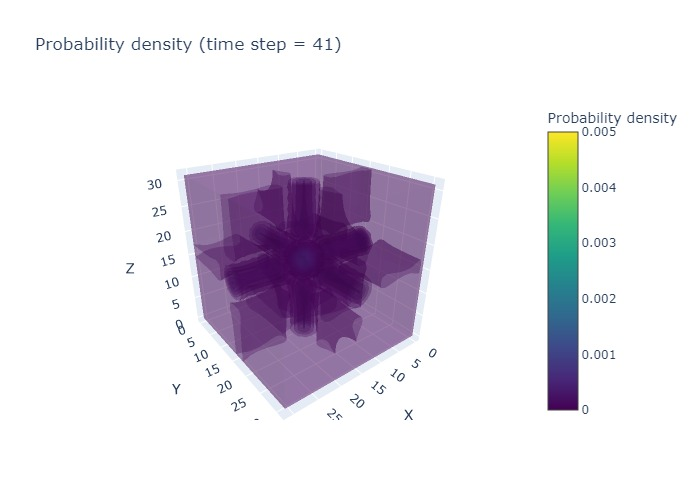
\includegraphics[width=0.75\textwidth]{"figures/interference_01.jpeg"}
	\caption{Unrealistic interference patterns as a result of DFT.}
	\label{fig:interference}
\end{figure}
This was the direct result of the way the used DFT transformation handles larger than zero values near the borders of the simulated volume.

To solve this problem we introduced a large potential barrier on each side of the simulated cube.
This wedged the probability density into the middle of the cube, where the potential remained zero.

